\let\negmedspace\undefined
\let\negthickspace\undefined
\documentclass[journal]{IEEEtran}
\usepackage[a5paper, margin=10mm, onecolumn]{geometry}
%\usepackage{lmodern} % Ensure lmodern is loaded for pdflatex
\usepackage{tfrupee} % Include tfrupee package

\setlength{\headheight}{1cm} % Set the height of the header box
\setlength{\headsep}{0mm}     % Set the distance between the header box and the top of the text

\usepackage{gvv-book}
\usepackage{gvv}
\usepackage{cite}
\usepackage{amsmath,amssymb,amsfonts,amsthm}
\usepackage{algorithmic}
\usepackage{graphicx}
\usepackage{textcomp}
\usepackage{xcolor}
\usepackage{txfonts}
\usepackage{listings}
\usepackage{enumitem}
\usepackage{mathtools}
\usepackage{gensymb}
\usepackage{comment}
\usepackage[breaklinks=true]{hyperref}
\usepackage{tkz-euclide} 
\usepackage{listings}
% \usepackage{gvv}                                        
\def\inputGnumericTable{}                                 
\usepackage[latin1]{inputenc}                                
\usepackage{color}                                            
\usepackage{array}                                            
\usepackage{longtable}                                       
\usepackage{calc}                                             
\usepackage{multirow}                                         
\usepackage{hhline}                                           
\usepackage{ifthen}                                           
\usepackage{lscape}
\usepackage{circuitikz}
\tikzstyle{block} = [rectangle, draw, fill=blue!20, 
    text width=4em, text centered, rounded corners, minimum height=3em]
\tikzstyle{sum} = [draw, fill=blue!10, circle, minimum size=1cm, node distance=1.5cm]
\tikzstyle{input} = [coordinate]
\tikzstyle{output} = [coordinate]


\begin{document}

\bibliographystyle{IEEEtran}
\vspace{3cm}

\title{12.213}
\author{AI25BTECH110031 \\ Shivam Sawarkar}
 \maketitle
% \newpage
% \bigskip
{\let\newpage\relax\maketitle}

\renewcommand{\thefigure}{\theenumi}
\renewcommand{\thetable}{\theenumi}
\setlength{\intextsep}{10pt} % Space between text and floats


\numberwithin{equation}{enumi}
\numberwithin{figure}{enumi}
\renewcommand{\thetable}{\theenumi}

\textbf{Question(12.213)}The set V of all polynomials of a real variable x of degree two or less and with real coefficients, constitutes a real linear vector space V = \{c0 + c1 x + c2 x2 : c0 , c1 , c2\} $\in$ $\mathbb{R}$ \\ 
\textbf{(a)} For $f(x) = a_0 + a_1x + a_2x^2 \in V$ and $g(x) = b_0 + b_1x + b_2x^2 \in V$, which one of the following constitutes an acceptable scalar product?

\begin{enumerate}[label=(\roman*)]
    \item $(f,g) = a_0^2b_0 + a_1^2b_1 + a_2^2b_2$
    \item $(f,g) = a_0^2b_0^2 + a_1^2b_1^2 + a_2^2b_2^2$
    \item $(f,g) = a_0b_0 - a_1b_1 + a_2b_2$
    \item $(f,g) = a_0b_0 + \dfrac{a_1b_1}{2} + \dfrac{a_2b_2}{3}$
\end{enumerate}

\textbf{(b)} Using the scalar product obtained in the above question, identify the subspace of $V$ that is orthogonal to $(1+x)$.

\begin{enumerate}[label=(\roman*)]
    \item $\{\, f(x) : b(1 - x) + c x^2,\, b,c \in \mathbb{R} \,\}$
    \item $\{\, f(x) : b(1 - 2x) + c x^2,\, b,c \in \mathbb{R} \,\}$
    \item $\{\, f(x) : b + c x^2,\, b,c \in \mathbb{R} \,\}$
    \item $\{\, f(x) : b x + c x^2,\, b,c \in \mathbb{R} \,\}$
\end{enumerate}


\textbf{Solution:} \\ 
Given,
\begin{align}
    V = \{\, a_0 + a_1x + a_2x^2 : a_i \in \mathbb{R} \,\}
\end{align}
is a real vector space. For
\begin{align}
f(x) = a_0 + a_1x + a_2x^2, \quad g(x) = b_0 + b_1x + b_2x^2,
\end{align}


A scalar product (inner product) $\langle f,g\rangle$ must satisfy: \\ 
1. Bilinearity, \\ 
2. Symmetry: $\langle f,g\rangle = \langle g,f\rangle$, \\ 
3. Positive definiteness: $\langle f,f\rangle > 0$ for all nonzero $f$.

Let us test each option:

\begin{align}
\begin{aligned}
\text{(i)} \quad & \langle f,g\rangle = a_0^2b_0 + a_1^2b_1 + a_2^2b_2 
&& \text{Not linear in } f. \\
\text{(ii)} \quad & \langle f,g\rangle = a_0^2b_0^2 + a_1^2b_1^2 + a_2^2b_2^2
&& \text{Not bilinear.} \\
\text{(iii)} \quad & \langle f,g\rangle = a_0b_0 - a_1b_1 + a_2b_2
&& \text{Not positive definite (e.g., for } f(x)=x). \\
\text{(iv)} \quad & \langle f,g\rangle = a_0b_0 + \frac{a_1b_1}{2} + \frac{a_2b_2}{3}
&& \text{Bilinear, symmetric, and positive definite.}
\end{aligned}
\end{align}

\begin{align}
\boxed{\text{Hence, (iv) is the acceptable scalar product.}}
\end{align}



Represent each polynomial $p(x) = a_0 + a_1x + a_2x^2$ by the coefficient vector
\begin{align}
\mathbf{a} = 
\begin{pmatrix} a_0 \\ a_1 \\ a_2 \end{pmatrix}.
\end{align}
The scalar product can be written as
\begin{align}
\langle f,g \rangle = \mathbf{a}^T D \mathbf{b}, \quad
D = \operatorname{diag}\!\left(1, \tfrac{1}{2}, \tfrac{1}{3}\right).
\end{align}
Then the orthogonality condition $\langle f, 1+x\rangle = 0$ becomes
\begin{align}
\mathbf{a}^T D \mathbf{u} = 0, \quad
\mathbf{u} = 
\begin{pmatrix} 1 \\ 1 \\ 0 \end{pmatrix}.
\end{align}
Compute
\begin{align}
D\mathbf{u} = 
\begin{pmatrix} 1 \\ \tfrac{1}{2} \\ 0 \end{pmatrix},
\quad
\Rightarrow
a_0 + \frac{a_1}{2} = 0.
\end{align}
\begin{align}
    \Rightarrow a_0=\frac{-a_1}{2}
\end{align}

and $a_2$ is independent \\
Let, $b=a_0$ and $c=a_2$
\begin{align}
    \vec{a}=b\myvec{1 \\ -2 \\ 0}+c\myvec{0 \\ 0 \\ 1}
\end{align}

So the orthogonal subspace is 2-dimensional with basis vectors corresponding to polynomials

\begin{align}
    1-2x, \quad x^2
\end{align}

Hence every polynomial orthogonal to  $1+x$ can be written 
\begin{align}
    b(1-2x)+cx^2
\end{align}

\begin{figure}
    \centering
    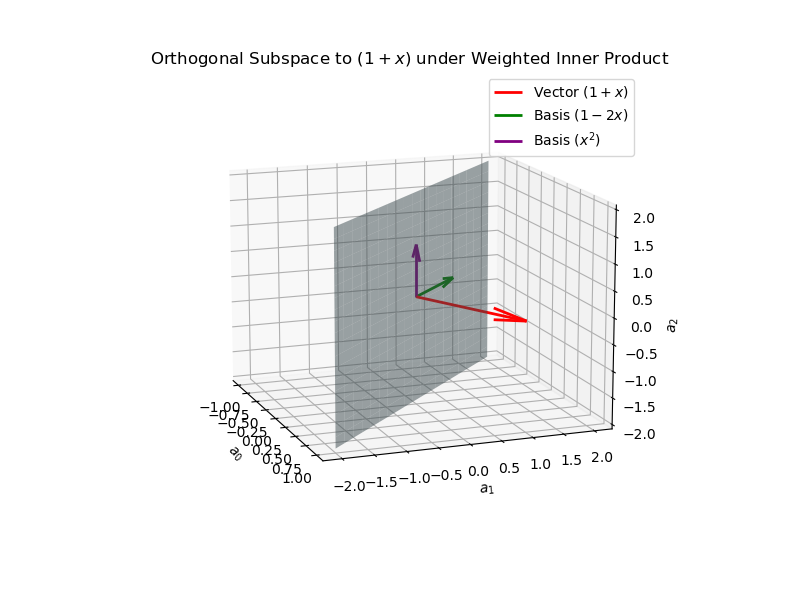
\includegraphics[width=1\linewidth]{Figs/Figure_1.png}
    \caption{}
    \label{fig:placeholder}
\end{figure}



\end{document}